\chapter{OpenModelica}
\thispagestyle{empty}
\label{chap11}

\section {Introduction}
OpenModelica (OM) is an open source modeling and simulation tool based on
Modelica language. Modelica is an object oriented language. As a result, it has all the
features of an object oriented language such as inheritance. Models or circuits are
defined in the form of classes, with in which there are components, functions,
connection and placement information. The OM suite has the following major tools.

\subsection {OMEdit}
An IDE for modeling and simulation. It supports a lot of electrical components. It
has a good graphical interface to drag and drop components and create the circuit.
One can only do transient simulation using this interface. An attractive feature of
OMEdit is the plotting interface. All the parameters in the circuit like voltages and currents through each component,
parameters like frequency, delay etc. will be displayed as
a list, after simulation. The user can choose the variables to be plotted in an
interactive manner from this list. On choosing the variable to plot, it will be plotted
on the plot window. One can also create multiple plot windows.

\subsection {OMOptim}
An IDE for optimisation. It lists all the variables in the given model. One can choose
the variables to be optimised from the list. Multiple models can be loaded for a given
optimisation problem. One can do multi objective optimisations as well. It supports
various optimisation algorithms such as Particle Swarm Optimisation (PSO) and
Simulated Annealing (SA). The results are displayed graphically.

\section {OpenModelica in eSim}
The above two functionalities can be accessed through the {\tt Modelica Converter} and {\tt OM Optimisation} tools on the eSim left toolbar. The two examples given below illustrates how to use OpenModelica in eSim. 

\subsubsection {Low Pass Filter circuit} 
Let us now see how to simulate a low pass filter in OpenModelica.
\begin{enumerate}
\item Open the schematic and create the circuit as shown in \figref{lowpass}. 

\begin{figure}[h]
\centering
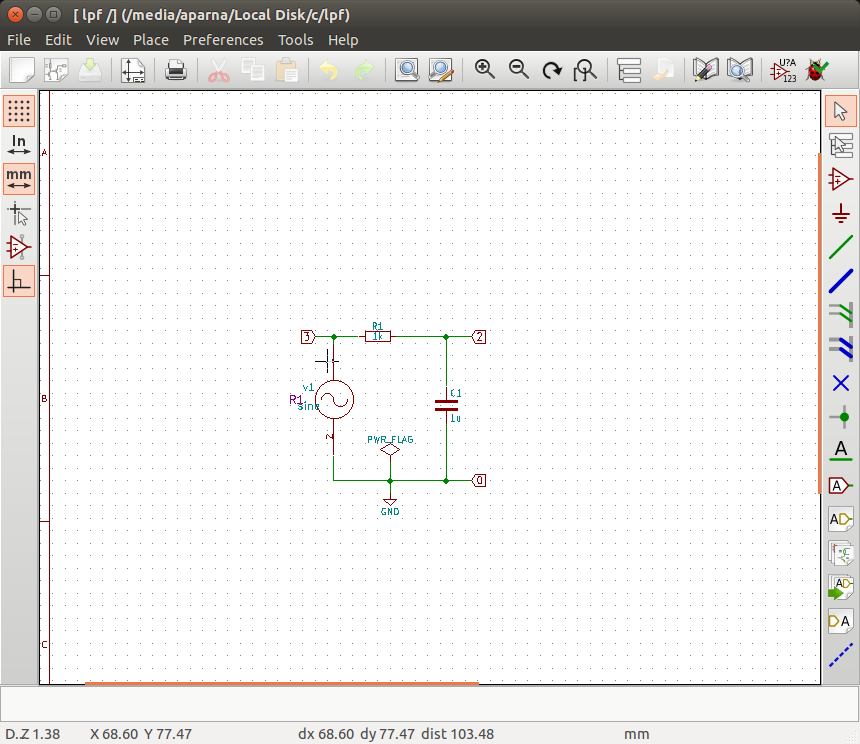
\includegraphics[width=\lgfig]{list_of_figures/1.png}
\caption{Circuit schematic: Low pass filter}
\label{lowpass}
\end{figure}

\item Create the KiCad netlist. Now the analysis and analysis parameters are given as shown in \figref{lowpass-analysis}. 

\begin{figure}[h]
\centering
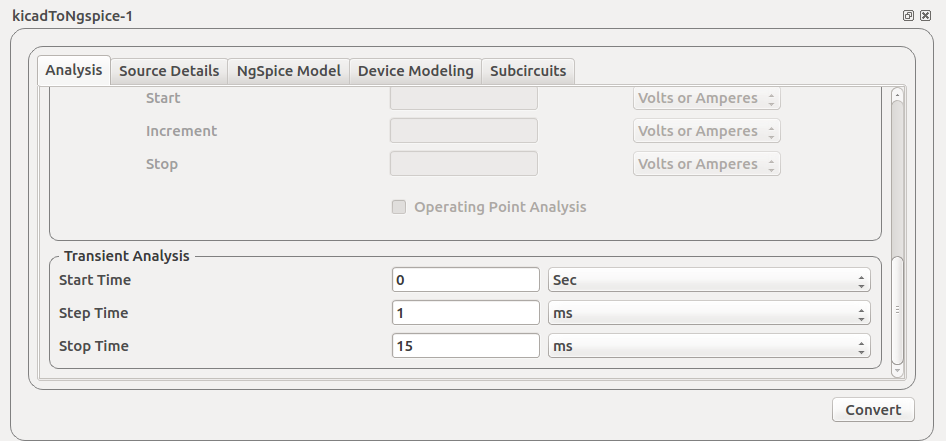
\includegraphics[width=\lgfig]{list_of_figures/2.png}
\caption{Analysis parameters: Low pass filter}
\label{lowpass-analysis}
\end{figure}

\item The source details are given as in \figref{lowpass-source}. The generated KiCad netlist is then converted to ngspice compatible netlist.

\begin{figure}[h]
\centering
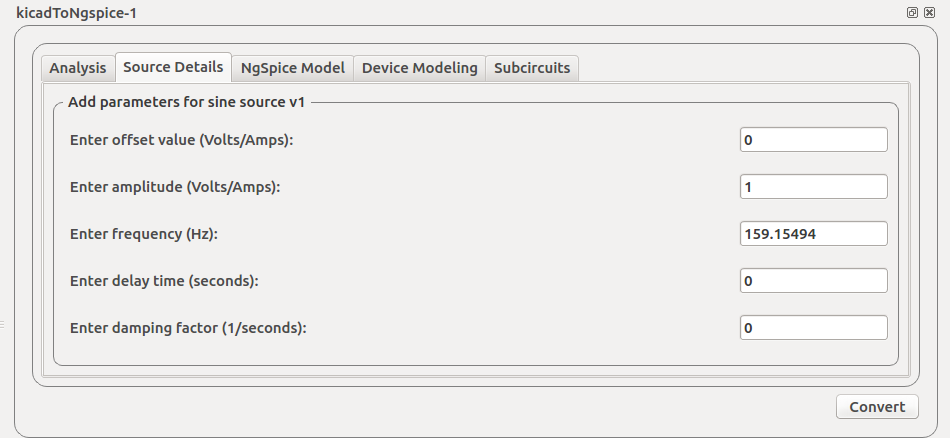
\includegraphics[width=\lgfig]{list_of_figures/3.png}
\caption{Source details: Low pass filter}
\label{lowpass-source}
\end{figure}

\item Simulate the ngspice netlist. The simulation curves are shown in \figref{lowpass-simulation}.

\begin{figure}[h]
\centering
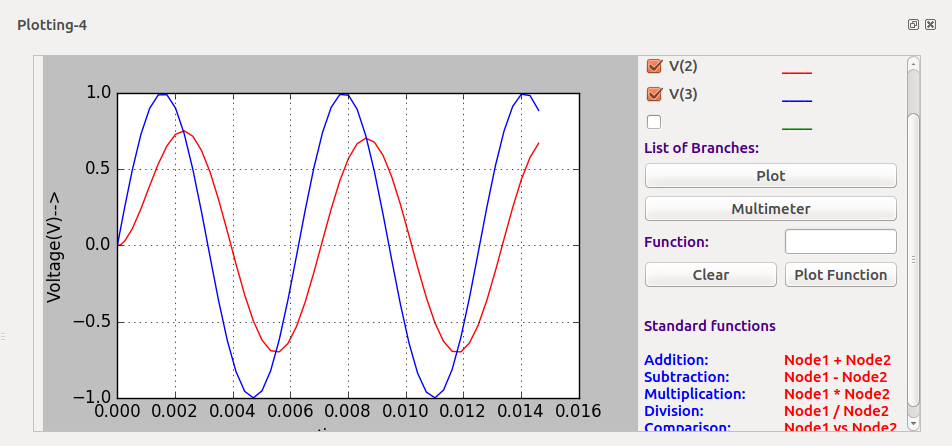
\includegraphics[width=\lgfig]{list_of_figures/4.png}
\caption{Simulation: Low pass filter}
\label{lowpass-simulation}
\end{figure}

\item Now to use OpenModelica, click on {\tt Modelica Converter} in the bottom left of eSim left toolbar.{\textit Make sure you have OpenModelica installed in the system}. This converter converts the spice netlist to Modelica format. Click on the LPF in the left that is appended in OpenModelica main window. Make sure you are in text view to see the Modelica code as shown in \figref{om-convert} Figure shows that LPF circuit is being used as a model, the initialisation of sources and components are in the beginning followed by the connection information. n3, n0,n2 are the nodes.

\begin{figure}[h]
\centering
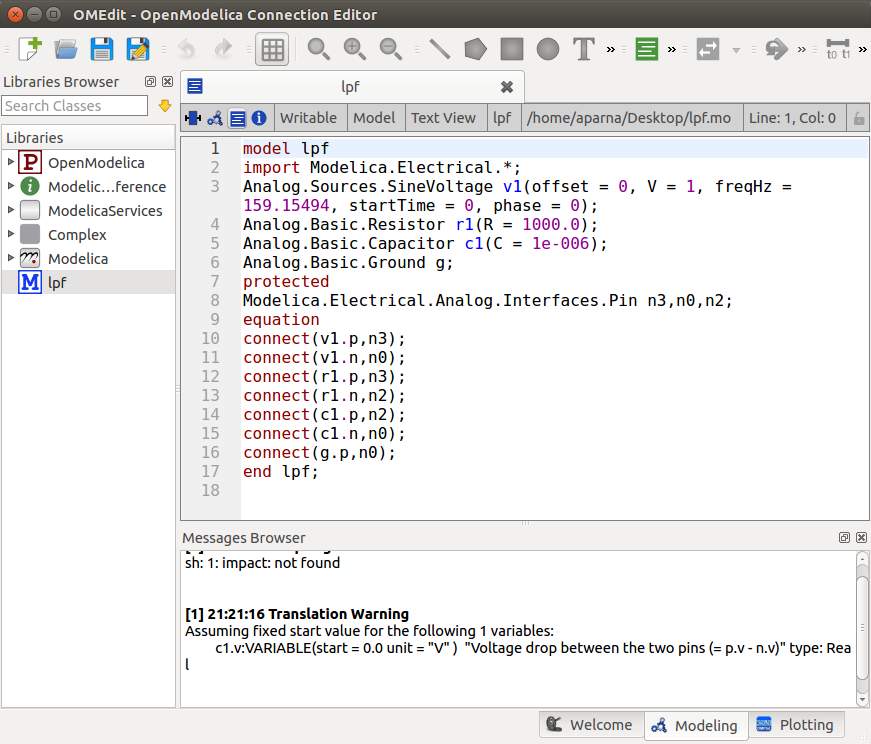
\includegraphics[width=\lgfig]{list_of_figures/5.png}
\caption{OpenModelica: Text view}
\label{om-convert}
\end{figure}

Default Modelica libary is used for electrical sources and components. This has to imported so that it can be used in the current circuit. This is available in the left side of main window. 

\item Click on Simulation Setup on the toolbar at the top. A window opens as shown in \figref{om-simsetup}. Give start and stop time. Click {\tt OK}.

\begin{figure}[h]
\centering
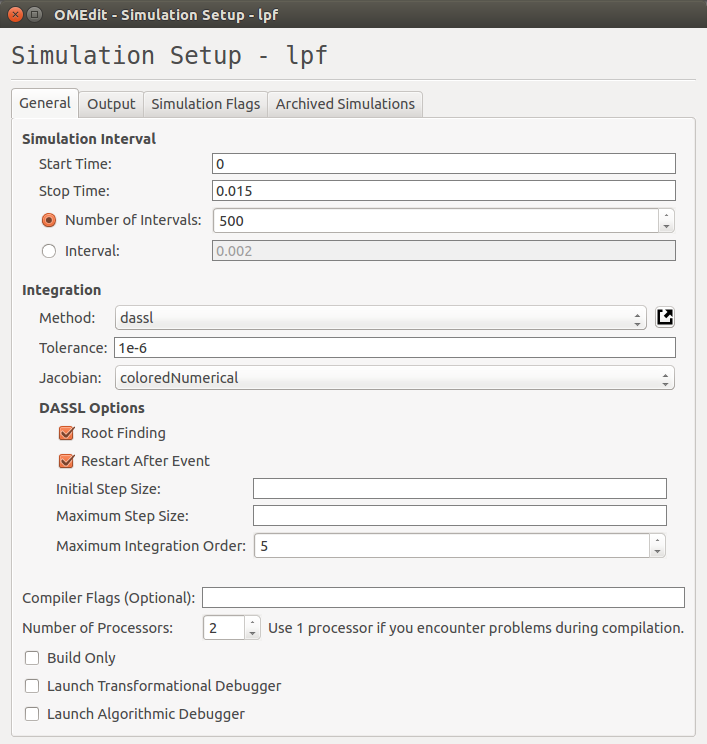
\includegraphics[width=\lgfig]{list_of_figures/6.png}
\caption{OpenModelica: Simulation setup}
\label{om-simsetup}
\end{figure}

\item A plotting window opens. Click on the node at the right to display the waveform. The window is shown in \figref{om-simulation}.

\begin{figure}[h]
\centering
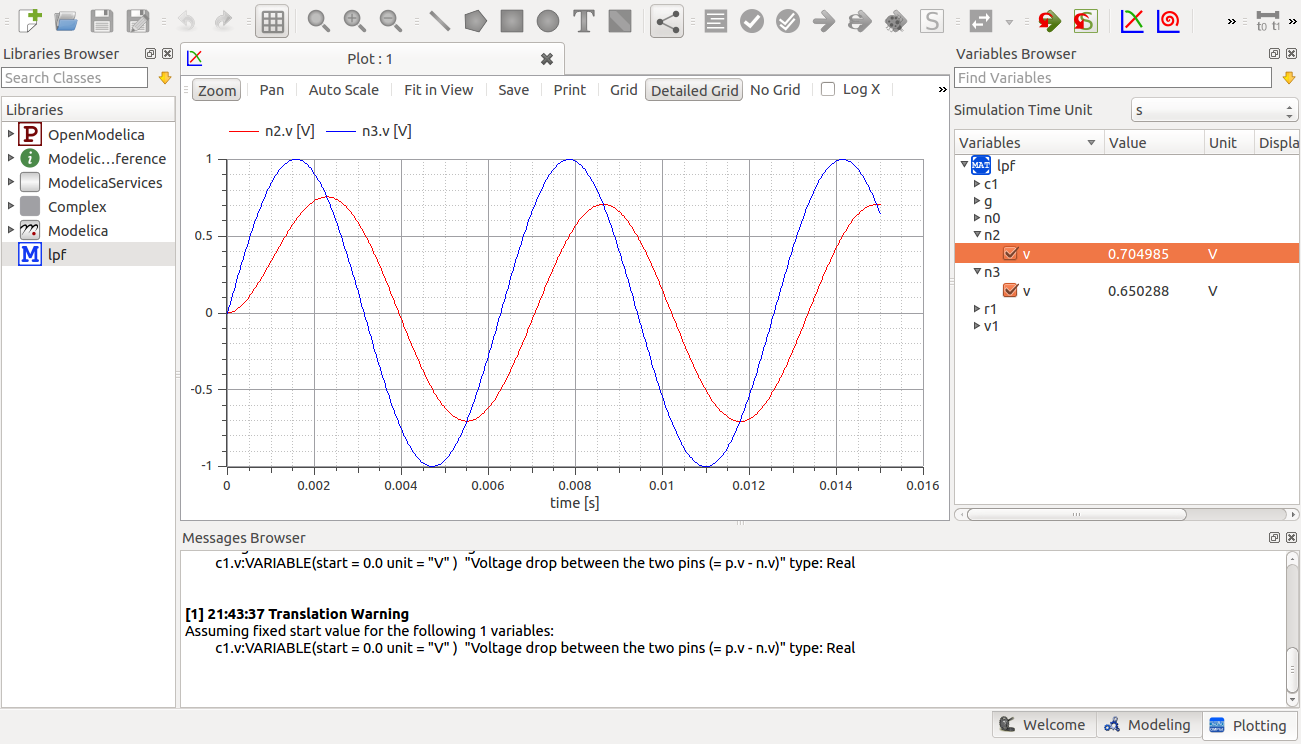
\includegraphics[width=\lgfig]{list_of_figures/7.png}
\caption{OpenModelica: Simulation}
\label{om-simulation}
\end{figure}

\end{enumerate}

\subsection {OM Optimisation}

Now let us explore how to use OpenModelica for optimisation through an example. Find the value of resistance R2 that maximises the power dissipated through it for the circuit in \figref{optim-circuit}. This is an illustration of the Maximum Power Transfer Theorem. The power is maximum when R2 = R1, i.e., when R2 = 100. So maximum power would be Pmax = 0.0625. Let us now see the steps to be followed find the value of R2 using eSim.

\begin{figure}[h]
\centering
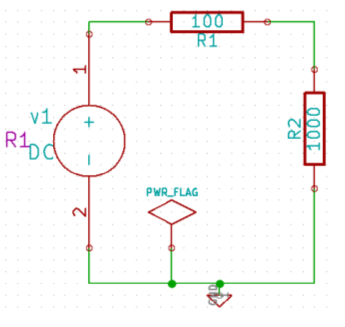
\includegraphics[width=\lgfig]{list_of_figures/8.png}
\caption{Circuit schematic for optimisation}
\label{optim-circuit}
\end{figure}

\begin{enumerate}
\item Follow all the steps as above and generate the Modelica model using the Ngspice to Modelica converter.

\item The objective function is $Power = i^2 \times R2$ . 
To define the objective function, the line $power := i^2 \times R1+ i^2 \times R2$  
is added under the keyword algorithm, in the Modelica model file.

\item Select {\tt OMOptim} from eSim left toolbar, in the displayed window click on {\tt New Project}. Then save the project. It is stored with an extension {\tt .min}. Now select {\tt Models} and then {\tt Load Modelica Library}. Now select {\tt Load mo file} under {\tt Models}. It will be added on the left. 

\item Click {\tt Problems} and then {\tt Optimisation}. Select the model to be optimised. \textit {Note that for optimising, that model has to be loaded in OpenModelica as stated before}. Clicking
blue turnover icon will display all the variables used in the model. Add details like optimsation variables and objective.

The OMOptim project for this problem is given in \figref{om-project}. Power is the objective function that has to be maximized. {\tt r2.R} is the variable that will be varied. {\tt r2.R} is limited between 0 and 1000.

\begin{figure}[h]
\centering
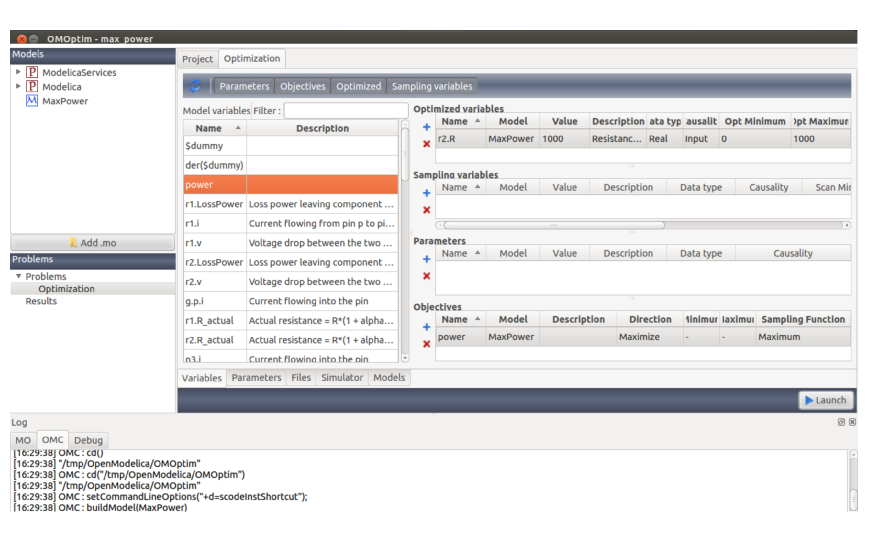
\includegraphics[width=\hgfig]{list_of_figures/9.png}
\caption{OMOptim project}
\label{om-project}
\end{figure}

\item Click on Parameters tab to select the type of algorithm and its parameters. In this example, the optimisation algorithm used is PSO (Particle Swarm Optimisation). The various parameter values given are as follows: population size as 50, Inertia factor as 1, Learning factor: alpha and beta as 2, Population saving frequency was 1. Iteration limit is also specified. Select the .mo file to be simulated from {\tt Files} tab. Click on {\tt Launch}. The results of optimisation for various values of Iteration Limit are given in \figref {table}.

\begin{figure}[h]
\centering
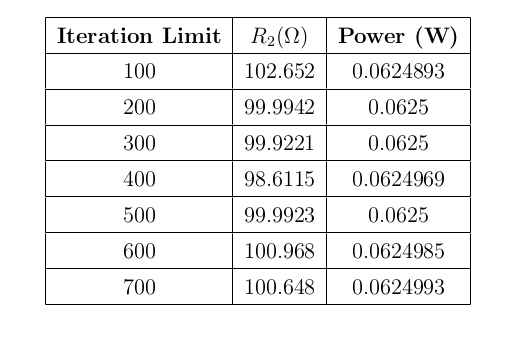
\includegraphics[width=\lgfig]{list_of_figures/10.png}
\caption{Optimisation values for various Iteration Limit }
\label{table}
\end{figure}

\item Depending on the type of algorithm, the time for optimisation varies. Optimised result is graphically displayed as shown in \figref {om-optimised}. 

\begin{figure}
\centering
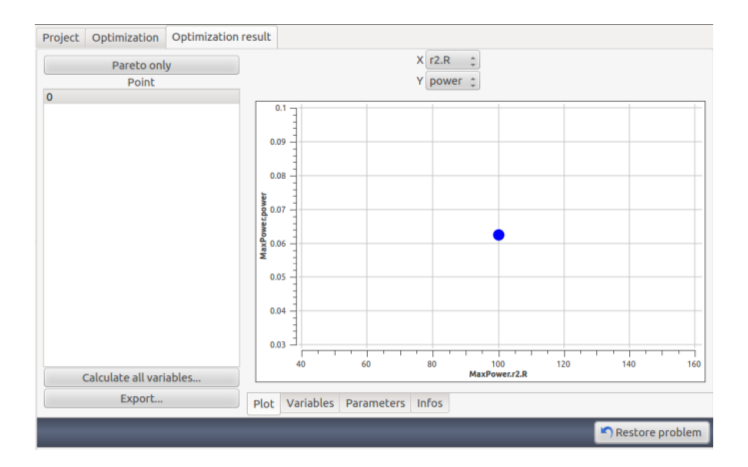
\includegraphics[width=\hgfig]{list_of_figures/11.png}
\caption{Optimised value of resistance for maximum power }
\label{om-optimised}
\end{figure}

\end{enumerate}

